\documentclass{article}\usepackage{amsmath,amssymb,amsthm,tikz,tkz-graph,color,chngpage,soul,hyperref,csquotes,graphicx,floatrow}\newcommand*{\QEDB}{\hfill\ensuremath{\square}}\newtheorem*{prop}{Proposition}\renewcommand{\theenumi}{\alph{enumi}}\usepackage[shortlabels]{enumitem}\usepackage[nobreak=true]{mdframed}\usetikzlibrary{matrix,calc}\MakeOuterQuote{"}\usepackage[margin=0.75in]{geometry} \newtheorem{theorem}{Theorem}

\title{EE16A - Lecture 14 Notes}
\author{Name: Felix Su$\quad$SID: 25794773}
\date{Spring 2016$\quad$GSI: Ena Hariyoshi}
\begin{document}
\maketitle

%%%% Topic %%%%
\subsection*{Switch Diagrams}
%%%% Notes %%%%
\begin{itemize}
    \item Analyze each phase of the diagram with one switched as ideal wires and off switches as open circuits
    \item Capacitors have no resistance in the scope of this class
    \item Total charge is conserved between switch phases
\end{itemize}
%%%% Topic %%%%
\subsection*{Charge Sharing}
%%%% Notes %%%%
\begin{itemize}
    \item Phase 1: Accumulate charge on variable capacitor
    \item Phase 2: Distribute charge between variable and fixed capacitor
    \begin{enumerate}
        \item Calculate total charge in Phase 1 ($C_{fix}$ should be 0, $C_{var}$ should be $Q$)
        \item Calculate total charge in Phase 2 in terms of $V_{out}$ ($Q_{fix} = C_{fix}V_{out}$, $Q_{var} = C_{var}V_{out}$)
        \item Equate two charges and solve for $V_{out}$
    \end{enumerate}
    \item Any resistor in a capacitor circuit will discharge capacitors
\end{itemize}
%%%% Topic %%%%
\subsection*{OpAmp}
%%%% Notes %%%%
\begin{center}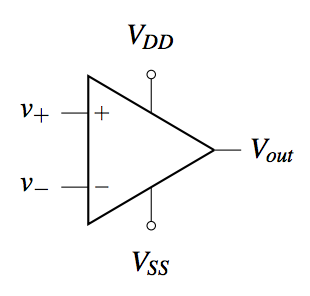
\includegraphics{op}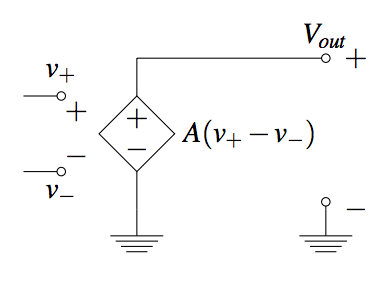
\includegraphics{opeq}\end{center}
\textbf{Example at (1:05:28)}
\begin{itemize}
    \item Equivalent to dependent voltage source that measures voltage between $V^+$ and $V^-$ (open circuit), and produces a voltage $V_{out}=A(V^{+}-V^{-})$
    \item Needs to be connected to 2 power sources ($V_{PP}=V_{DD}, V_{NN}=V_{SS}$)
    \item $A$ is ideally an infinite scale factor, which would theoretically cause infinite $V_{out}$, but $V_{out}$ is restricted to the range of ($V_{SS} = V_{NN} < V_{out} < V_{DD} = V_{PP}$)
\end{itemize}
\begin{mdframed}
\textbf{OpAmp Equations and Properties:}
\begin{itemize}
    \item 5 terminals: $V^+, V^-, V_{out}, V_{DD}, V_{SS}$
\end{itemize}
\begin{equation}V_{out}=A(V^{+}-V^{-})\end{equation}
\begin{equation}V_{SS} < V_{out} < V_{DD}\end{equation}
\end{mdframed}
%%%% Topic %%%%
\subsection*{Capacitor Touch Screen}
%%%% Notes %%%%
\textbf{Variable Capacitance:}
\begin{itemize}
    \item Determines if finger has touched
    \begin{enumerate}
        \item Charge variable capacitor to a fixed voltage
        \item Because $Q = CV$, capacitance varies, and voltage is fixed, charge $Q$ now varies.
        \item Move varying $Q$ onto another fixed capacitor (parallel)
        \item Because $V = \frac{Q}{C}$, $Q$ varies, and $C$ is fixed, this is the varying voltage
    \end{enumerate}
\end{itemize}
\textbf{Using an OpAmp}
\begin{center}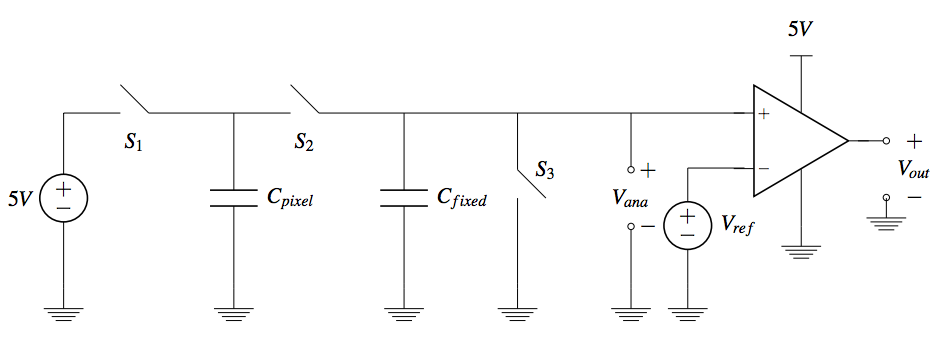
\includegraphics{cts}\end{center}
\begin{itemize}
    \item Purpose:
    \begin{enumerate}
        \item Takes analog voltage created by switch/capacitor system, and force it to be either $0V$ or $5V$
        \item Uses an open circuit with infinite resistance (no voltage drop/current)
    \end{enumerate}
    \item Want $V_{out}$ to be $V_{max}$ on touch, and $0$ on no touch
\end{itemize}
\textbf{Detecting Finger Touch}
\begin{center}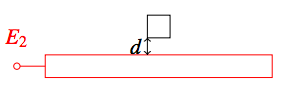
\includegraphics{2d1}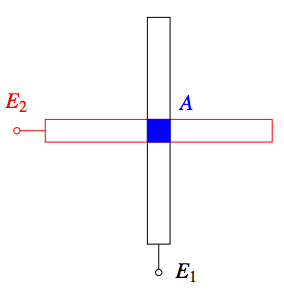
\includegraphics{2d2}\end{center}
\begin{center}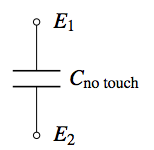
\includegraphics{cnt}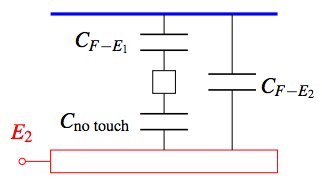
\includegraphics{ct}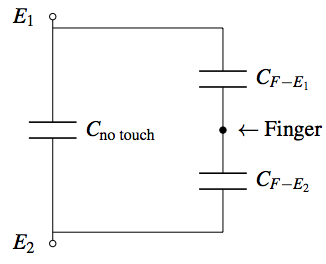
\includegraphics{ctcd}\end{center}
\begin{itemize}
    \item Pixel is intersection of capacitors
    \item Connect charge sharing parallel capacitors to OpAmp:
    \begin{itemize}
        \item $V_{var} = V_{ana} = V^+$, $V_{ref} = V^-, V_{DD} = V_{max}$, $V_{SS} =$ ground $= 0$
        \item Choose $V_{ref}$ and $C_{fix}$ s.t. $V_{ana} > V_{ref}$ on touch, and $V_{ana} < V_{ref}$ when not touching
        \begin{itemize}
            \item OpAmp forces $V_{DD}$ and $V_{SS}$
        \end{itemize}
        \item $C_{notouch}$ is $\frac{\varepsilon A}{d}$ : 1 capacitor between $(E_1, E_2)$
        \item $C_{touch}$ is $C_{notouch} + (C_{fin}, E_1)||(C_{fin}, E_2)$ : finger adds two more capacitors in parallel
    \end{itemize}
\end{itemize}
\begin{mdframed}
\begin{equation}C_{notouch} = \frac{\varepsilon A}{d}\end{equation}
\begin{equation}C_{touch} = C_{notouch} + (C_{fin}, E_1)||(C_{fin}, E_2)\end{equation}
\end{mdframed}
\end{document}
